\documentclass{standalone}
\usepackage{pgfplots}
\usepackage{tikz}
\usepackage{amsmath}
\pgfplotsset{compat=1.16}

\begin{document}

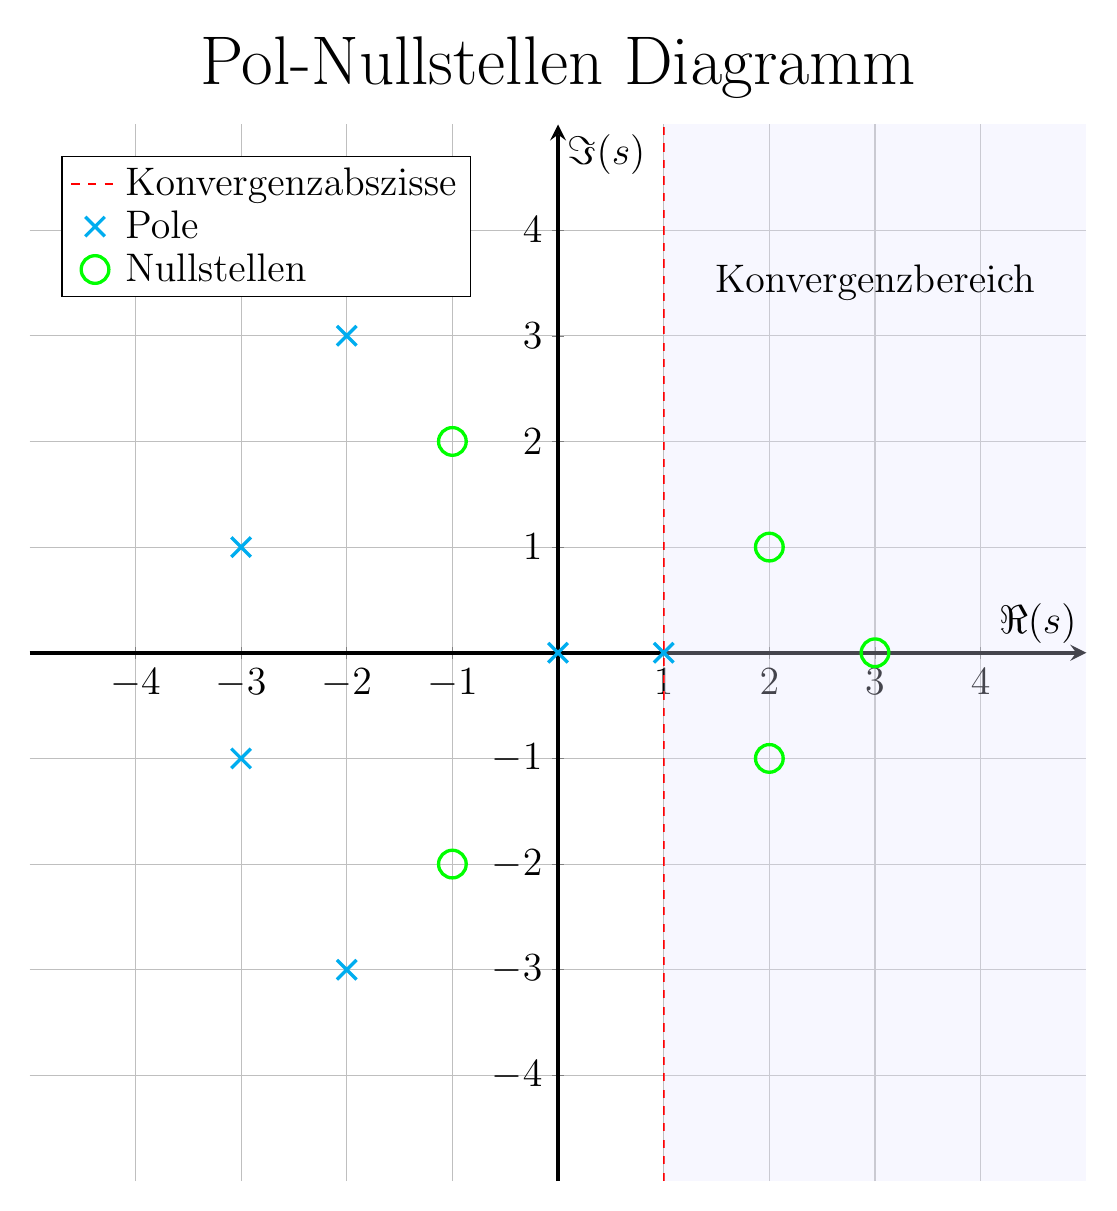
\begin{tikzpicture}[very thick, scale=1, font=\Large]
\begin{axis}[
    width=15cm, height=15cm,
    title=\Huge{Pol-Nullstellen Diagramm},
    xlabel=$\Re(s)$, ylabel=$\Im(s)$,
    xmin=-5, xmax=5, ymin=-5, ymax=5,
    axis lines=center,
    xtick={-4,-3,...,4}, ytick={-4,-3,...,4},
    grid=major,
    legend pos=north west, legend cell align=left,
    axis line style={line width=1.5pt}
]

% Konvergenzabszisse
\addplot[red, thick, dashed] coordinates {(1,-5) (1,5)};
\addlegendentry{Konvergenzabszisse}

% Pole
\addplot[cyan, very thick, only marks, mark=x, mark size=5pt] coordinates {
    (-2,3) (-2,-3) (-3,1) (-3, -1) (0,0) (1,0)
};
\addlegendentry{Pole}

% Nullstellen
\addplot[green, very thick, only marks, mark=o, mark size=5pt] coordinates {
    (-1,2) (-1,-2) (3,0) (2, 1) (2, -1)
};
\addlegendentry{Nullstellen}

% Konvergenzbereich
\fill[blue!10, opacity=0.3] (1,-5) rectangle (5,5);
\node at (3,3.5) {Konvergenzbereich};

\end{axis}
\end{tikzpicture}

\end{document}
